%%%%%%%%%%%%%%%%%%%%%%% file template.tex %%%%%%%%%%%%%%%%%%%%%%%%%
%
% This is a template file for Web of Conferences Journal
%
% Copy it to a new file with a new name and use it as the basis
% for your article
%
%%%%%%%%%%%%%%%%%%%%%%%%%% EDP Science %%%%%%%%%%%%%%%%%%%%%%%%%%%%
%
%%%\documentclass[option]{webofc}
%%% "twocolumn" for typesetting an article in two columns format (default one column)
%
\documentclass{webofc}
\usepackage[varg]{txfonts}   % Web of Conferences font

\usepackage{hyperref}

\usepackage{pgfgantt}
\usepackage{capt-of}
\usepackage{listings}

\lstset{
  frame=single,                    % frame around the code
  %numbers=left,                   % where to put the line-numbers
  stepnumber=1,                   % the step between two line-numbers.
  numbersep=5pt,                  % how far the line-numbers are from the code
  backgroundcolor=\color{white},  % choose the background color. You must add \usepackage{color}
  showspaces=false,               % show spaces adding particular underscores
  showstringspaces=false,         % underline spaces within strings
  showtabs=false,                 % show tabs within strings adding particular underscores
  tabsize=2,                      % sets default tabsize to 2 spaces
  captionpos=b,                   % sets the caption-position to bottom
  breaklines=false,                % sets automatic line breaking
  breakatwhitespace=true,         % sets if automatic breaks should only happen at whitespace
}


%
% Put here some packages required or/and some personnal commands
%
%
\begin{document}

%
\title{dCache integration with CERN Tape Archive}
%
% subtitle is optionnal
%
%%%\subtitle{Do you have a subtitle?\\ If so, write it here}

\author{
         \firstname{Tigran} \lastname{Mkrtchyan}\inst{1}\fnsep\thanks{\email{tigran.mkrtchyan@desy.de}} \and
        \firstname{Jacek} \lastname{Chodak}\inst{1}\fnsep \and
        \firstname{Mwai} \lastname{Karimi}\inst{1}\fnsep \and
        \firstname{Ralf} \lastname{Lueken}\inst{1}\fnsep \and
        \firstname{Svenja} \lastname{Meyer}\inst{1}\fnsep \and
        \firstname{Peter} \lastname{Suchowski}\inst{1}\fnsep \and
        \firstname{Christian} \lastname{Voss}\inst{1}\fnsep
}

\institute{
Deutsches Elektronen-Synchrotron DESY, Notkestrasse 85, 22607 Hamburg, Germany
}

\abstract{%
  The ever-increasing amount of data that is produced by modern scientific facilities like EuXFEL or LHC puts
  high pressure on the data management infrastructure at the laboratories. This includes poorly shareable resources
  of archival storage, typically, tape libraries. To achieve maximal efficiency of the available tape resources, a
  deep integration between hardware and software components is required. The CERN Tape Archive (CTA) is an open-source storage management system developed by CERN to manage LHC experiment
  data on tape. Although today CTA's primary target is CERN Tier-0, the data management group at DESY considers the
  CTA as a main alternative to commercial HSM systems. dCache has an extensible tape interface that allows connectivity to almost any tape system. Together with the CERN Tape Archive developers, the storage team at DESY is working on seamless integration of CTA into dCache.
}
%
\maketitle
%
\section{Introduction}
\label{intro}

The ever-increasing amount of data that is produced by modern scientific facilities like EuXFEL or LHC puts high pressure
on the data management infrastructure at the laboratories. The challenges that have to be addressed span the full data 
life-cycle: from ingest and efficient data analysis up to long-term preservation. The latter typically utilizes magnetic
tape media, which in combination with disk storage covers the data management requirements. DESY-IT groups use dCache\cite{dcache}, a
storage system developed at DESY in collaboration with Fermilab and Nordic eInfrastructure Collaboration (NeIC), to manage
large numbers of disk servers and transparent data migration to and from archival storage.

Even though today large hard disk-based storage systems are cost, space and volume-effective (1 PB disk storage requires less than a ${1m^{3}}$ of space),
magnetic tapes are still the best option for long-term data archiving, especially for so-called cold data (data that are rarely accessed).
Indeed, tape cartridges don't require electric power when not used, can store up to 20TB of uncompressed data and are designed for
15 - 30 years of archival storage. To organize a large number of tape cartridges, tape libraries with robotic arms are used.

There are, of course, some drawbacks to tape-based technologies. When streaming, a modern tape drive provides up to 400 MB/s
and the so-called positioning time on average is about 50 seconds. This doesn't include the mount time, the time which is needed by the
robotic arm to put the tape into an appropriate tape drive. Moreover, magnetic tapes don't support concurrency, which means that only
one stream, i.e., only one file, can be read or written at any point in time.

Thus, to achieve maximal efficiency of the available tape resources, i.e., to minimize the number of tape (re)mounts and maximize the time during which tape is read or written at
maximal speed, a deep integration between hardware and software components is required.

Since the early 90's, DESY-IT has been relying on Open Storage Manager (OSM) software to operate tape libraries and access data on tapes\cite{osm_desy}.
During these three decades, the OSM underwent many changes. Over 80\% of the original code base has been updated to address computer, network,
operating system and software paradigms that have changed over the decades. Nevertheless, the scaling capabilities put into the original design
don't apply today. Moreover, the commercial software license of OSM doesn't allow us to share our changes with the broader scientific community.
As a result, a new scalable and preferably open-source successor is required.

With dCache as the primary disk layer in front of an HSM, the tape system should fulfil the following requirements:

\begin{itemize}
    \item maximization of tape HW efficiency, as mentioned above,
    \item integration into DESY ecosystem,
    \item integration with dCache tape interface,
    \item support for Enterprise\footnote{Enterprise tape media refers to high-capacity vendor-specific magnetic tapes, for example, IBM TS1170\cite{ibm_ts1170}} \& LTO\footnote{Linear Tape-Open (LTO) - is an open tape standard defined by LTO Consortium\cite{lto_consortium} formed by IBM, HP and Seagate} media types,
    \item daily turnover of about 1PB, as expected during PETRA-IV operation,
    \item stable operation for the next decade,
    \item open-source, adopting open standards,
    \item wide user and technology community,
    \item state-of-the-art integration/use development tools (CI/CD).
\end{itemize}

Of course, some of those requirements heavily depend on end-user workflow. For example, the data file size has a great influence on the tape read/write performance, as bigger files are more suitable for data streaming, while small files often require tape repositioning. As tape drives can be accessed only by a single stream at a time, the concurrent store and restore requests to single tapes are serialized, and the concurrent store and/or restore requests to different tapes are limited by the number of available tape drives. Writing data to multiple tapes increases overall write throughout, but requires multiple tape mounts on reads.

\section{Cern Tape Arcive}
\label{sec:cta}

The CERN Tape Archive (CTA)\cite{cta} is an open-source storage system developed by the CERN IT storage group to
replace the legacy CASTOR system that is used to manage the experiments' data on tapes. Its architecture is designed
to meet the requirements of LHC Run 3 as well as HL-LHC, thus meeting the requirements of the most data-intensive scientific workloads.

The CTA has two key components: frontend and tape daemon (Fig. \ref{fig:cta_overview}). The frontend accepts requests, like archive, retrieve, delete or cancel, from the attached disk storage and puts them into a request queue. If needed, the file catalogue is updated. The scheduling logic is embedded into the tape daemons, which are per-tape drive processes that seek matching tasks in the request queue. Once the desired number of requests is collected, the data are moved between disk and tape media using an embedded xroot\cite{xrootd} client.

\begin{figure}[h]
    \centering
    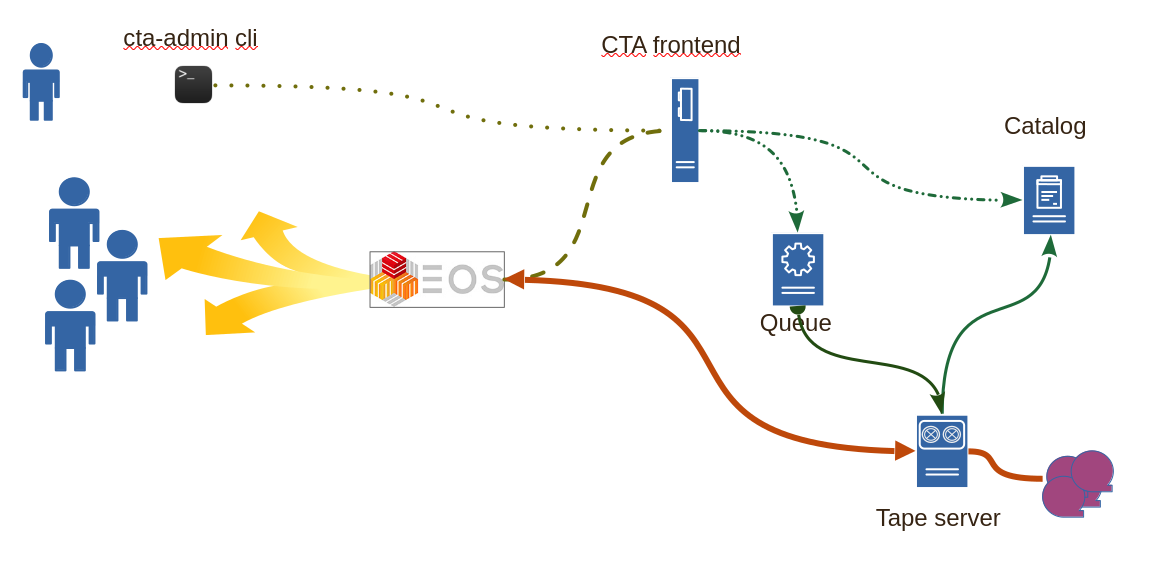
\includegraphics[scale=0.25]{cta-design.png}
    \caption{CTA design overview}
    \label{fig:cta_overview}
\end{figure}

Out of the box, CTA comes with a frontend that communicates with EOS, the disk system deployed at CERN. However, as CTA's queuing system is not EOS aware, other frontend implementations are possible. Moreover, the CTA project is actively working on flexibility in the system to allow wider adoption by other sites, ease of contributions from other developers and elimination of CERN-specific dependencies in the provided binary packages \cite{cta_beyond_cern}.

To trigger data migration between disk and tape, CTA supports two request types: \textit{Archive} and \textit{Retrieve}. The retrieve operation can be cancelled with a \textit{Cancel Retrieve} request. The \textit{Delete} request is used to cancel the archive operation or/and to remove an existing file from the tape catalogue. In the case of the EOS disk frontend, all those operations are tied to EOS filesystem events, like \textit{CREATE}, \textit{CLOSE}, \textit{READ} and \textit{DELETE}. The requests are encoded with Google's protobuf \cite{prtobuf} and sent from EOS server to CTA frontend over the Xroot Scalable Service Interface (XrootdSSI). In addition to data migration requests, the frontend supports operations required by the admin-cli tool, like \textit{define tape pool} or \textit{enable/disable tape drive}.

The CTA scheduler queue is backed by the CEPH\cite{ceph} object store or by a shared filesystem. This allows hundreds of thousands of requests to be collected for optimal scheduling decisions.

\section{dCache Integration with CTA}
\label{sec:integration}

dCache has a flexible tape interface which allows connectivity to any tape system. There are two ways that a file can be migrated to tape. Either dCache calls an HSM-specific copy command or it interacts with the tape system via an in-dCache HSM-specific driver, called a nearline storage provider. The latter has been shown (by NDGF, TRIUMF and KIT Tier-1s), to provide better resource utilization and efficiency\cite{endit_kit}. The achieve seamless integration with CTA the dCache developers at DESY have therefore implemented a CTA-specific nearline storage provider, called dcache-cta\cite{dcache_cta}, and a corresponding frontend component for CTA. The communication between dCache and the new frontend is based on Google’s gRPC library.

\begin{lstlisting}[label=grpc-frontend,caption={gRPC service definition},keywords={service,rpc,returns}]
    service CtaRpc
    {
      rpc Create (Request) returns (CreateResponse) {}
      rpc Archive (Request) returns (ArchiveResponse) {}
      rpc Retrieve (Request) returns (RetrieveResponse) {}
      rpc Delete (Request) returns (Empty) {}
      rpc CancelRetrieve (Request) returns (Empty) {}
      rpc Version (Empty) returns (Version) {}
    }
\end{lstlisting}

The gRPC-based service is limited to data migration operations, so the XrootdSSI-based frontend is needed to provide admin-tool functionality\footnote{There is ongoing development to migrate the admin interface to a gRPC-based\cite{grpc} frontend. This activity is not directly correlated to dCache with CTA integration.}.

As CTA has its own scheduler, to avoid double scheduling,  the flush and restore request queuing at the dCache pools should be disabled. In this way, all HSM requests from dCache are directly submitted to the CTA scheduler.

\begin{figure}[h]
    \centering
    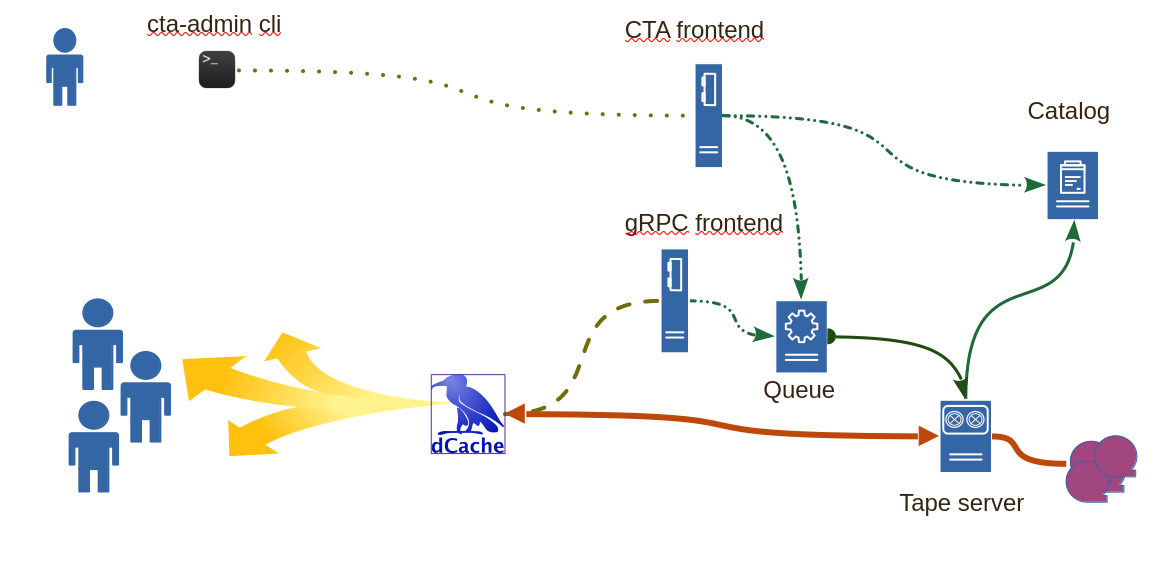
\includegraphics[scale=0.25]{dcache-cta-integration.png}
    \caption{dCache integration with CTA}
    \label{fig:dcache_integration}
\end{figure}

\section{Migration from OSM}
\label{migraion}

DESY has a long history of providing HSM interfaces for scientific data. Today we have about 170PB on the tape media. Obviously, the migration to CTA should avoid physical file copies from one tape to another and be performed only by conversion of the existing OSM database schema to the CTA catalogue format. The migration procedure was split into three steps:
\begin{itemize}
    \item database schema migration,
    \item update of CTA tape server to support OSM-formated tapes,
    \item update of file HSM-related metadata in dCache with CTA-relevant reference.
\end{itemize}

To add OSM tape format support to CTA, the CTA catalogue was extended to understand 
which format is used by a particular tape. This information is then propagated to the tape servers, which use a format-specific reader\footnote{Writing in the old format is not supported and all migrated tapes are marked as read-only.}.

Despite the fact that OSM and CTA have completely different high-level designs, both system catalogues are pretty similar (Fig.\ref{fig:osm_entry_example} and Fig.\ref{fig:cta_entry_example}) and require very few adjustments during the schema migration.

\begin{figure}[h]
    \centering
    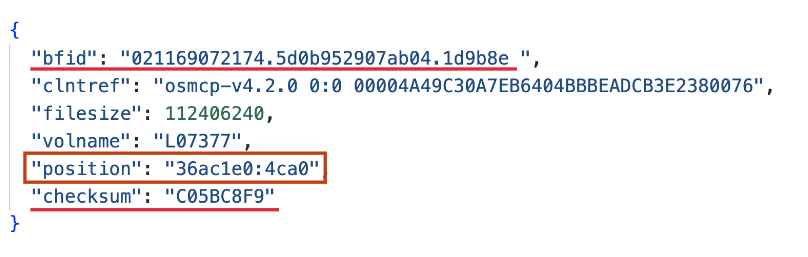
\includegraphics[scale=0.60]{osm-schema.png}
    \caption{Example of file metadata in the OSM catalogue.}
    \label{fig:osm_entry_example}
\end{figure}

\begin{figure}[h]
    \centering
    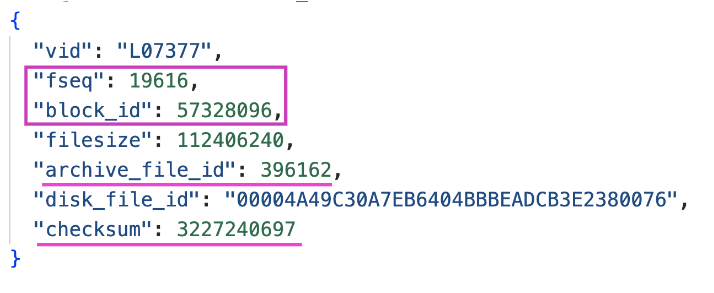
\includegraphics[scale=0.60]{cta-schema.png}
    \caption{Example of file metadata in the CTA catalogue.}
    \label{fig:cta_entry_example}
\end{figure}

The link between files stored in dCache and their location on a tape relies on a so-called \textit{HSM-URI} - a URL that specifies the HSM type with an HSM type-specific identifier, opaque for dCache, that is generated by the HSM when data are written to tape:

~\\
tape location $\Rightarrow$ $\begin{cases}
    osm://<instance>/111.222.333 &\text{for } OSM \\
    cta://<instance>/archiveid=123 &\text{for } CTA
\end{cases}$
~\\

dCache automatically will use the correct HSM setup based on the HSM-type in the tape location URI.

Since dCache can support multiple tape systems in parallel, the migration from OSM to CTA is performed experiment by experiment. As of today (August 2023), almost all experiments have already migrated and newly created data is being written to tape with CTA.

\section{First operational experience}
\label{experence}

The current deployment at DESY provides a single CTA instance shared between all dCache instances. We use four LTO-9 or IBM TS1160 tape drives attached per single tape server node. The hosts are equipped with 100 Gb/s, which is more than sufficient for the system's theoretical maximum streaming rate of 12.8Gb/s (4 x 400 MiB/s). During operation, the observed average drive speed was around 350MiB/s.  An NFS-mounted volume is used as the backend for the scheduler queue and easily handles a large number of archive and restore requests.

Based on our experience with dCache and OSM, the CTA instance at DESY uses the PostgreSQL database\cite{postgres} as a backend for catalogue implementation. We run PostgreSQL in hot stand-by mode to ensure the system's reliability and performance.

\begin{figure}[h]
    \centering
    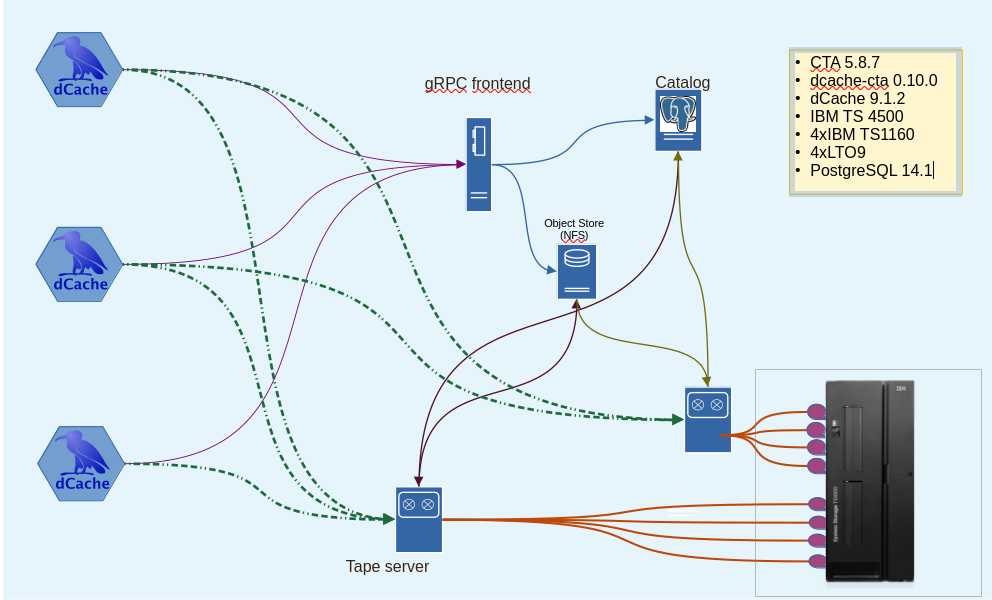
\includegraphics[scale=0.30 ]{cta-deployment-desy.png}
    \caption{dCache with CTA. Deployment at DESY}
    \label{fig:dcache_cta_deplyment}
\end{figure}

The biggest challenge for the operational team was(is) the differences with existing OSM installations. Despite the fact that CTA deployment is simpler to operate\footnote{This is of course a subjective impression of the team members.}, new unfamiliar error situations have been observed. During the first month of operation, many modifications to the dcache-cta and cta-grpc-frontend have been applied. For example, we added an option to control the number of gRPC server threads, that process incoming requests on the CTA frontend; implemented dCache $\leftrightarrow$ CTA communication timeout; increased dCache internal HSM request lifetimes; and updated the number of open file descriptors to match the number of gRPC requests. We anticipate that this list will expand as our experience with CTA continues to mature.


\section{Summary and future work}
\label{summary}

Today, we are pretty confident that dCache+CTA will address the data archival requirements of HEP, Photon Science and EuXFEL at DESY. The system has proven to provide the expected data rates and functionality. The migration from OSM to CTA was started in the spring of 2023 and is expected to be completed by the end of 2023.

CTA's open-source development style allows the DESY team to actively contribute to the project. All changes that are required to run dCache with CTA are part of the standard dCache builds (starting from dCache version 7.2) and public CTA releases (starting from 5.7.12). The setup at DESY is replicated by PIC in Barcelona and Fermilab, in the USA. Both sites currently run Enstore\cite{enstore} and plan to migrate to dCache+CTA in 2024.
 
The new gRPC-based interface has proven its simplicity and functionality and is under evaluation by the EOS-CTA team for adoption.

Both CTA and dCache projects are rapidly changing to match the requirements of the scientist. To avoid regressions, all software releases are intensively tested for interoperability. However, today the testing of CTA $\leftrightarrow$ dCache integration is a manual operation, thus error-prone and not scalable. The automatization of such test procedures is essential for catching defects early in the development cycle and ensuring software quality.

\newpage
\bibliography{bibliography}
\end{document}
